
% Global variables for the whole document
\title{Recherche du partenaire supersymétrique du quark top et mesure des propriétés des dépôts dans le trajectographe à pistes de silicium de l’expérience CMS au Run 2}
\author{Mark\'{e}ta Jansov\'{a}}
\date{27 Septembre 2018}

% Geometry for the title page only
\newgeometry{top=3cm, bottom=2.5cm, left=2cm, right=2cm, bindingoffset=0cm}

\begin{textblock}{0}[0,0](0.25,0.5)
{
    \setlength{\fboxsep}{0.7pt}
    \setlength{\fboxrule}{1pt}
    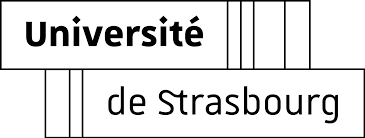
\includegraphics[height=1.5cm]{figures/lunistra}
}
\end{textblock}

\begin{textblock}{0}[0,0](12.5,0.5)
{
    \setlength{\fboxsep}{0.7pt}
    \setlength{\fboxrule}{1pt}
    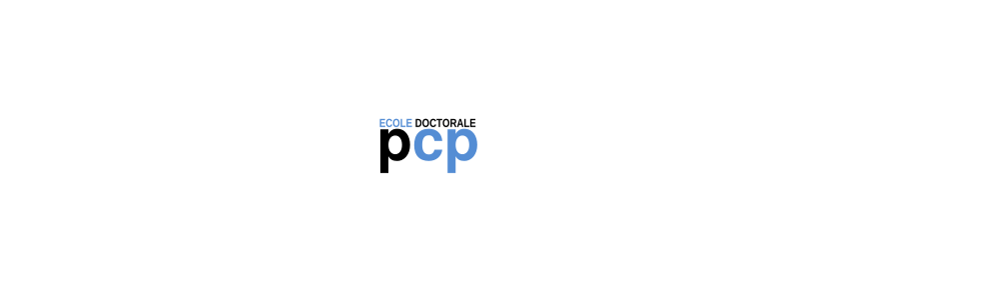
\includegraphics[height=1.5cm]{figures/logoED}
}
\end{textblock}

\begin{titlepage}
    \begin{center}
    \vspace*{-2cm}
        {\Large \textbf{UNIVERSITÉ DE STRASBOURG}}\\

        \vspace*{1cm}

        {\large \textbf{ÉCOLE DOCTORALE DE PHYSIQUE ET CHIMIE PHYSIQUE}}\\
        \textbf{Institut Pluridisciplinaire Hubert Curien}\\

        \vspace*{1cm}

        {\LARGE \textbf{TH\`{E}SE}} présentée par:

        \vspace*{0.3cm}

        {\Large \textbf{Mark\'{e}ta JANSOV\'{A}}}

        soutenue le: \textbf{27 Septembre 2018}
        

        \vspace*{1cm}

        pour obtenir le grade de: \textbf{Docteur de l'université de Strasbourg}


        Discipline/Spécialité: Physique des particules


        \vspace*{1cm}

        \fbox{
        \parbox{\textwidth}{\centering \LARGE \textbf{Recherche du partenaire supersymétrique du quark top et mesure des propriétés des dépôts dans le trajectographe à pistes de silicium de l’expérience CMS au Run 2}} %}
%\centering
         }

        \end{center}

        \vspace*{1cm}

        {\large \textbf{THÈSE dirigée par:}}\\
        \begin{tabular}{ll}
        \hspace{1cm}    \textbf{Mme. COLLARD Caroline}          & Institut Pluridisciplinaire Hubert Curien \\
        \end{tabular}
        
        {\large \textbf{RAPPORTEURS:}} \\
        \begin{tabular}{ll}
            \hspace{1cm}    \textbf{M. KAJFASZ Éric~~~~~~~~}                & Centre de Physique des Particules de Marseille\\
            \hspace{1cm}    \textbf{M. TROCME Benjamin}             & Laboratoire de Physique Subatomique \& Cosmologie \\
        \end{tabular}
        \vspace*{0.5cm}
        \hline

        \vspace*{0.5cm}
        {\large \textbf{AUTRES MEMBRES DU JURY:}}\\
        \begin{tabular}{ll}
            \hspace{1cm}    \textbf{Mme. BOUDOUL Gaëlle~~}            & Institut de Physique Nucléaire de Lyon \\
            \hspace{1cm}    \textbf{M. BAUDOT Jérôme}               & Institut Pluridisciplinaire Hubert Curien, Unistra \\
            \hspace{1cm}    \textbf{M. CHABERT Éric}                & Institut Pluridisciplinaire Hubert Curien, Unistra \\
        \end{tabular}

        \vspace*{0.5cm}

    \vspace*{1cm}
\end{titlepage}
\restoregeometry
